\documentclass[10pt,conference,a4paper]{IEEEtran_EDM}
\IEEEoverridecommandlockouts
% The preceding line is only needed to identify funding in the first footnote. If that is unneeded, please comment it out.
% \usepackage{cite}
\usepackage{amsmath,amssymb,amsfonts}
\usepackage{algorithmic}
\usepackage{graphicx}
\usepackage{textcomp}
\usepackage{xcolor}

\usepackage{biblatex}
\addbibresource{sources.bib}

\def\BibTeX{{\rm B\kern-.05em{\sc i\kern-.025em b}\kern-.08em
    T\kern-.1667em\lower.7ex\hbox{E}\kern-.125emX}}


\def\confheader{}

\makeatletter
\newcommand{\linebreakand}{%
  \end{@IEEEauthorhalign}
  \hfill\mbox{}\par
  \mbox{}\hfill\begin{@IEEEauthorhalign}
}
\makeatother

\usepackage{flushend} % <------------- used for automatically balance the columns on the last page. Be careful, read HOWTO XIV. LAST PAGE COLUMN EQUALIZATION 

\begin{document}

\markboth{\confheader}{}
\title{Python RANSAC Library for Common Objects}
\author{
\IEEEauthorblockN{line 1: 1\textsuperscript{st} Egor Skorobogatov}
\IEEEauthorblockA{\textit{line 2: dept. name of organization}\\ 
\textit{(of Affiliation)} \\
\textit{line 3: name of organization}\\ 
\textit{(of Affiliation)}\\
line 4: City, Country \\
line 5: email address or ORCID}
\and
\IEEEauthorblockN{line 1: 2\textsuperscript{nd} Robert Vakhnenko}
\IEEEauthorblockA{\textit{line 2: dept. name of organization}\\ 
\textit{(of Affiliation)} \\
\textit{line 3: name of organization}\\ 
\textit{(of Affiliation)}\\
line 4: City, Country \\
line 5: email address or ORCID}
\and
\IEEEauthorblockN{line 1: 3\textsuperscript{rd} Pyotr Grimalyuk}
\IEEEauthorblockA{\textit{line 2: dept. name of organization}\\ 
\textit{(of Affiliation)} \\
\textit{line 3: name of organization}\\ 
\textit{(of Affiliation)}\\
line 4: City, Country \\
line 5: email address or ORCID}

\linebreakand  % <------------- and with a line-break

\IEEEauthorblockN{line 1: 4\textsuperscript{th} Given Name Surname}
\IEEEauthorblockA{\textit{line 2: dept. name of organization}\\ 
\textit{(of Affiliation)} \\
\textit{line 3: name of organization}\\ 
\textit{(of Affiliation)}\\
line 4: City, Country \\
line 5: email address or ORCID}
\and
\IEEEauthorblockN{line 1: 5\textsuperscript{th} Given Name Surname}
\IEEEauthorblockA{\textit{line 2: dept. name of organization}\\ 
\textit{(of Affiliation)} \\
\textit{line 3: name of organization}\\ 
\textit{(of Affiliation)}\\
line 4: City, Country \\
line 5: email address or ORCID}
\and
\IEEEauthorblockN{line 1: 6\textsuperscript{th} Given Name Surname}
\IEEEauthorblockA{\textit{line 2: dept. name of organization}\\ 
\textit{(of Affiliation)} \\
\textit{line 3: name of organization}\\ 
\textit{(of Affiliation)}\\
line 4: City, Country \\
line 5: email address or ORCID}
}

\maketitle


\begin{abstract}

RANSAC is one of the most popular and important algorighms in computer vision.
It is being used in robotics, medical imaging and many more fields. Also,
python is one of the most frequently used languages at the moment, especially
in computer vision. In spite of the facts above, the options for a python
library for RANSAC that works out of the box are very limited. This paper is
about starkit-ransac -- a python package with algorithms for detecting most of
the common objects. In this work, firstly we go over alternatives: pyRANSAC-3D
and scuf. We look at their advantages and disadvantages and how we can improve
on existing solutions. Secondly, we present our own solution -- starkit-ransac
-- a batteries-included python library for RANSAC. Third, we compare this
library to it's alternatives via benchmarks and ease of use. In short, this
package is significantly faster on some shapes that are included in pyRANSAC-3D
and a bit slower, but more modular than scuf.

\end{abstract}

\begin{IEEEkeywords}
RANSAC, python, computer vision, detection, library, package
\end{IEEEkeywords}

\section{Introduction}
RANSAC is a computer vision algorightm that is quite simple: 
\begin{enumerate}
    \item take some samples from the dataset,
    \item build a hypothesis from these samples,
    \item check this hypothesis' quality on the whole dataset,
    \item select the best hypothesis.
\end{enumerate}
This algorithm provides robust detection of objects and that is what gives it
it's popularity. Having a package that already contains some basic objects that
are used frequently and acts as a framework would be quite useful in many
fields, such as robotics. At the moment, despite RANSAC's ubiquity, there are
no python packages that satisfy these conditions. Thus, a python package that
is modular, contains, all the basic shapes and works out of the box is
presented.

\section{Previous Works}
During research on available solutions, we found a lot and very few at the same
time. Scipy\cite{2020SciPy-NMeth} presents a ransac algorithm for linear
regression, and some other solutions present RANSAC for homography and
fundamental matrix \cite{Mishkin2015MODS}. However, there are just two
prominent libraries for RANSAC on points clouds:
pyRANSAC-3D\cite{Mariga_pyRANSAC-3D_2022} and scuf\cite{SCUF}. These packages
do some things well, but we believe, that we could improve on them.

\subsection{pyRANSAC-3D}
pyRANSAC-3D \cite{Mariga_pyRANSAC-3D_2022} is a python package
pyRANSAC-3D contains all the basic shapes: 
\begin{itemize}
    \item line,
    \item plane,
    \item circle in space,
    \item cuboid(intersection of three perpendicular planes),
    \item cylinder
\end{itemize}
This is a good set of objects that may be used almost anywhere and this package
is really simple to use out-of-the-box.

However, this package has some critical issues. Firstly, it has remained
unmaintained since 2022, so no new shapes were added and chances are, they will
not be. Also, this library's code for circle in space contains a severe bug
that prevents correct detection. Other significant drawback that we would like
to improve on is modularity. pyRANSAC-3D is effectively a collection of RANSAC
scripts without any overarching structure, so adding a new shape is not as
simple as it could be. And lastly, this library's code for fitting can be sped
up, as shown in %todo: add speedup.


\subsection{scuf}
Another solution that we found was SCUF -- Spheroid Consensus Undeterministic
Fitting. This is a package that implements fitting for all the quadrics --
surfaces that are described by equation \eqref{eq:quadric-eq}.
\begin{equation}
    (x-c)^T Q (x-c) = 1,
    \label{eq:quadric-eq}
\end{equation}
where $x$ is any point that lies on a given surface, $c$ is a vector that
typically is the center of the shape and $Q$ is a matrix that encapsulates
rotation and radii of the shape.
It is worth noticing that \eqref{eq:quadric-eq} can be expanded to
\eqref{eq:quadric-expanded} which also covers line and plane in 3d, and circle
and ellipsoid in 2d.
\begin{multline}
    A x^2 + B y^2 + C z^2 + D xy + \\+ E xz + F yz + G x + H y + I z + J = 0
    \label{eq:quadric-expanded}
\end{multline}

The approach that SCUF uses allows for a faster hypothesis score estimation
beacuse it can easily be vectorized. SCUF's RANSAC works like this:
\begin{enumerate}
    \item create a list of all sample sets iterations,
    \item create a list of hypothesis models for each sample set,
    \item estimate all models in one go, by applying \eqref{eq:quadric-expanded}
        to the whole dataset.
\end{enumerate}
This allows for a very fast fitting, because using one numpy\cite{numpy} matrix
operation is much faster than using it multiple times. At the same time, this
approach limits this implemetation only to shapes that can be easily expressed
in closed form. Thus, one of the goals that we strive for is making our library
more flexible and allowing for any shape.

Another problem of this library is that despite having some code for all the
shapes listed above, it seems that only ellipsoid works. This library provides
no acces to RANSAC fitting of any shapes except ellipsoid, ellipse, plane and
line in 2D. Ellipsoid detection works quite well, and it's implemetation is
quite efficient, as will be shown %todo: add speed comparison
. This, however, cannot be said for ellipse, plane and line2d. scuf's RANSAC
for these surfaces may work fine, but no acces to it is provided directly.

\section{Library Structure}

\subsection{Goals}
As stated before, we aim to create a library that is easy to use
out-of-the-box, allows for modification and contains frequently used shapes.

As for shapes, the goal was to implement RANSAC for the following objects:
\begin{enumerate}
    \item circle in 2D,
    \item ellipse in 2D,
    \item line in 3D,
    \item plane in 3D,
    \item circle in 3D,
    \item sphere,
    \item ellipsoid
\end{enumerate}
Also, two other objects were implemented: a staircase and M\"obius strip.

To achieve ease of use, we decided, that we would create and interface for each
surface that would be used in RANSAC. It should be easy to implemet shapes, so
we decided to create a single interface for surfaces.

To properly test all the shapes, it was decided, that starkit-ransac should
have a generation module. All generation functions should be able to add noise
and generate any surface based on a model and generate any surface based on a
model.

Another consideration for ease of use was visualization. We decided that we
should implement a visualization module that would allow for visualization of
any fit shape included in starkit-ransac.

And lastly, we strived to use as little external libraries as possible.
Surfaces, RANSAC algorithm and data generation only use one external dependency
and it is numpy. Visualization requires open3d, but it is not required for
fitting.

\subsection{Architecture}
It is only natural to semantically split entities into three categories:
RANSAC, surfaces and utility. RANSAC category contains everything that is
directly related to the algorithm. Surfaces category contains an abstract
surface class, that provides an interface for any surface. And obviously, it
contains all the surfaces themselves. Utility is self-explanatory.
Besides, to make this library more convenient to use, we decided to implement
synthetic data generation and visualization for our surfaces. These are two
other categories, that we will discuss later.

At the very start, it was decided to implement an abstract surface model class, which
would later serve as a template. This class provides an interface for the main
RANSAC implementation and has the following attributes:
\begin{itemize}
    \item num\_samples -- a field that tells how many samples of data are
        required to build a single model,
    \item fit\_model -- a method that accepts samples and set's it's instance
        class' parameters to the ones described by samples,
    \item calc\_distances -- a method that accepts a list of points and returns
        a list of distances from these points to the surface.
\end{itemize}
This interface allows to write a single RANSAC class that than can be used to
detect any surface that has these attributes. At same time, this design has
it's drawbacks. For example, it can't be vectorized easily. In general case, it
is impossible to calculate all distances for all models using a single dot
product or something similar.

Second, we implemeted a basic RANSAC class. One of the considerations was that
user may want to detect different objects on the same point cloud. Therefore, a
RANSAC class may be initialized with a set of points and points may be added
later. As of now, this class present only one way to fit and sample, however
it's implementation allows for easy modification and addition of other methods
of scoring or sampling. As a result, this class return a fit object, that can
be used for visualization, data generation etc.

Generation module generates any number of point for any model passed to it with
any standard deviation. It allows for easy comparison with a perfect model and
allows for easy testing.

%todo: add open3d
Another stated goal is visualization. One of the most convenient tools for this
purpose is open3d\cite{open3d} library. Visualization module contains functions
to visualize all the objects. All visualization functions accept a model as
their input parameter and return something that can be directly drawn via
open3d.

\section{Comparison}

\subsection{Benchmarking setup}
Our library includes a test suite to validate all the shapes on different sets
of data. Also, it creates multiple sets of test data that can be repurposed and
used in other scenarios. To benchmark and compare the results, we decided to
set a fixed number of 500 RANSAC iterations and fixed distance threshold of 0.1
for all shapes. Benchmarking was conducted using pytest\_benchmark plugin for
pytest. We evaluated the time required to fit a model including hypothesis
evaluation and sampling, i.e. one full RANSAC run.

Since shapes included in starkit-ransac and other libraries are not the same,
we benchmarked only those shapes that were available in at least one of other
libraries. We compared pyRANSAC-3D's fitting with ours on the following shapes:
line, plane, circle in 3D and sphere. scuf was benchmarked only on ellipsoid
and sphere. 

\subsection{Benchmark results}
%todo: add figures
As shown on figure~\ref{fig:comparison}, we can see that starkit-ransac is much
faster that pyRANSAC-3D on fitting a line and circle in 3D. We believe that
line fitting is this much faster because of a better distance evaluation that uses no

\begin{figure}
    \begin{center}
        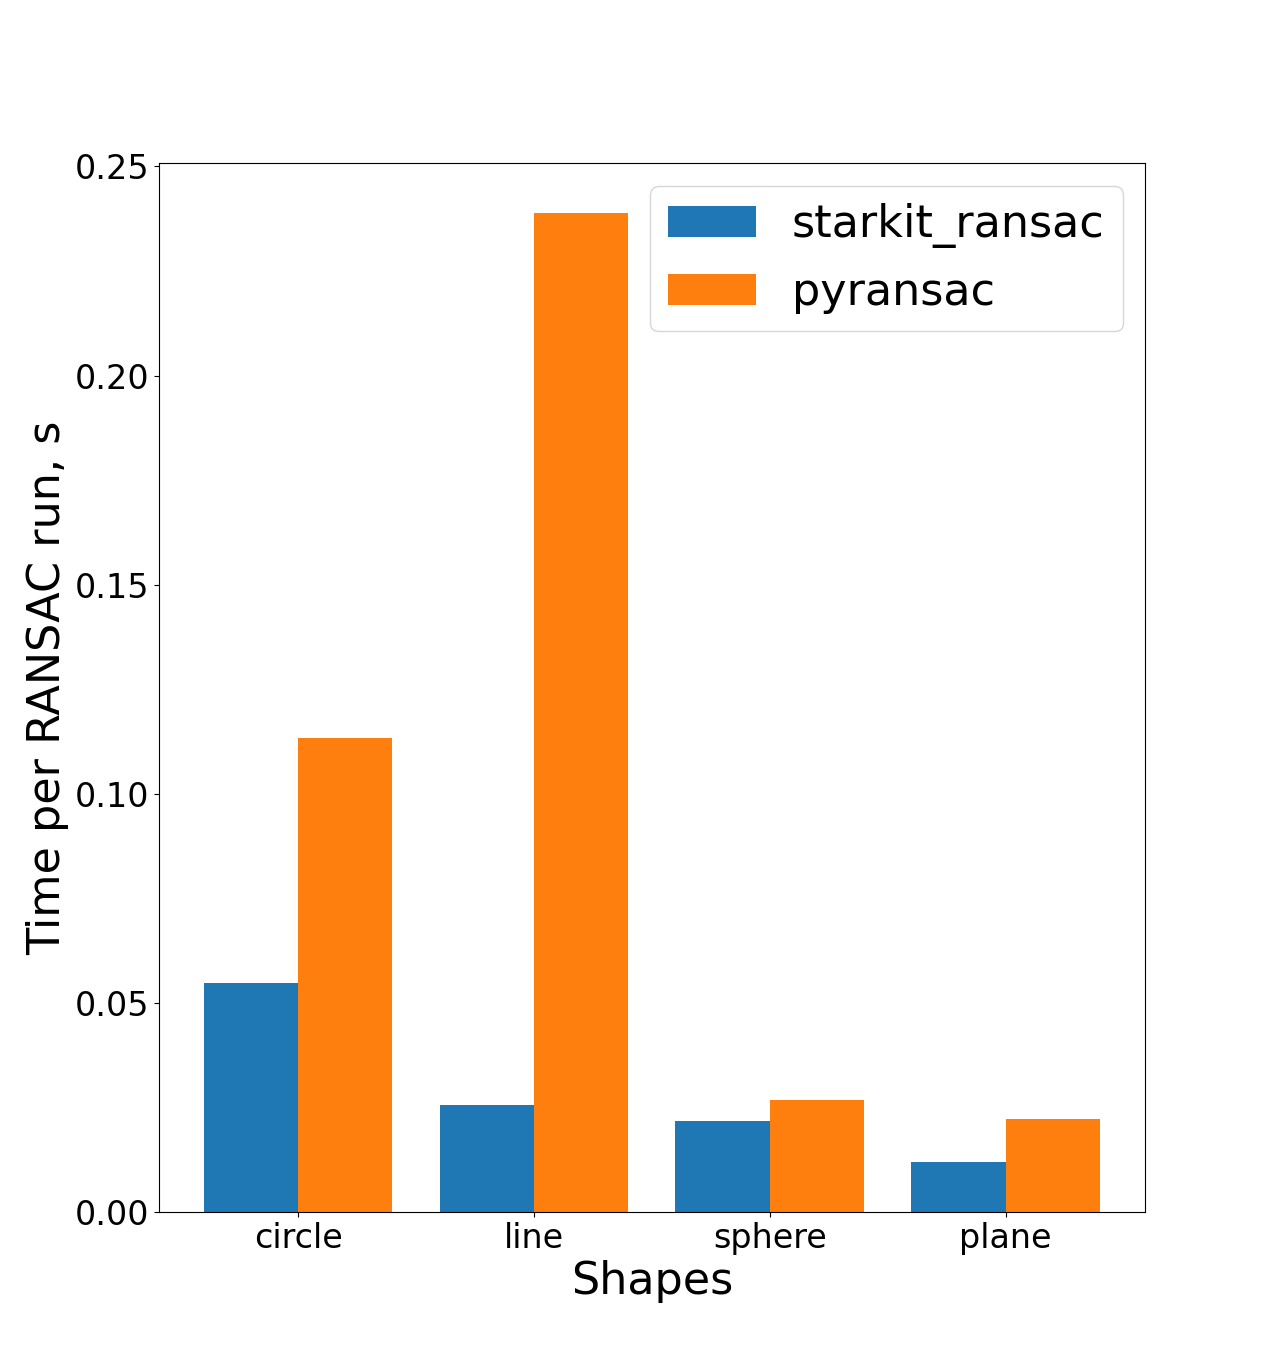
\includegraphics{figures/pyransac-comparison.png}
    \end{center}
    \caption{}\label{fig:comparison}
\end{figure}

\begin{figure}[htbp]
\centerline{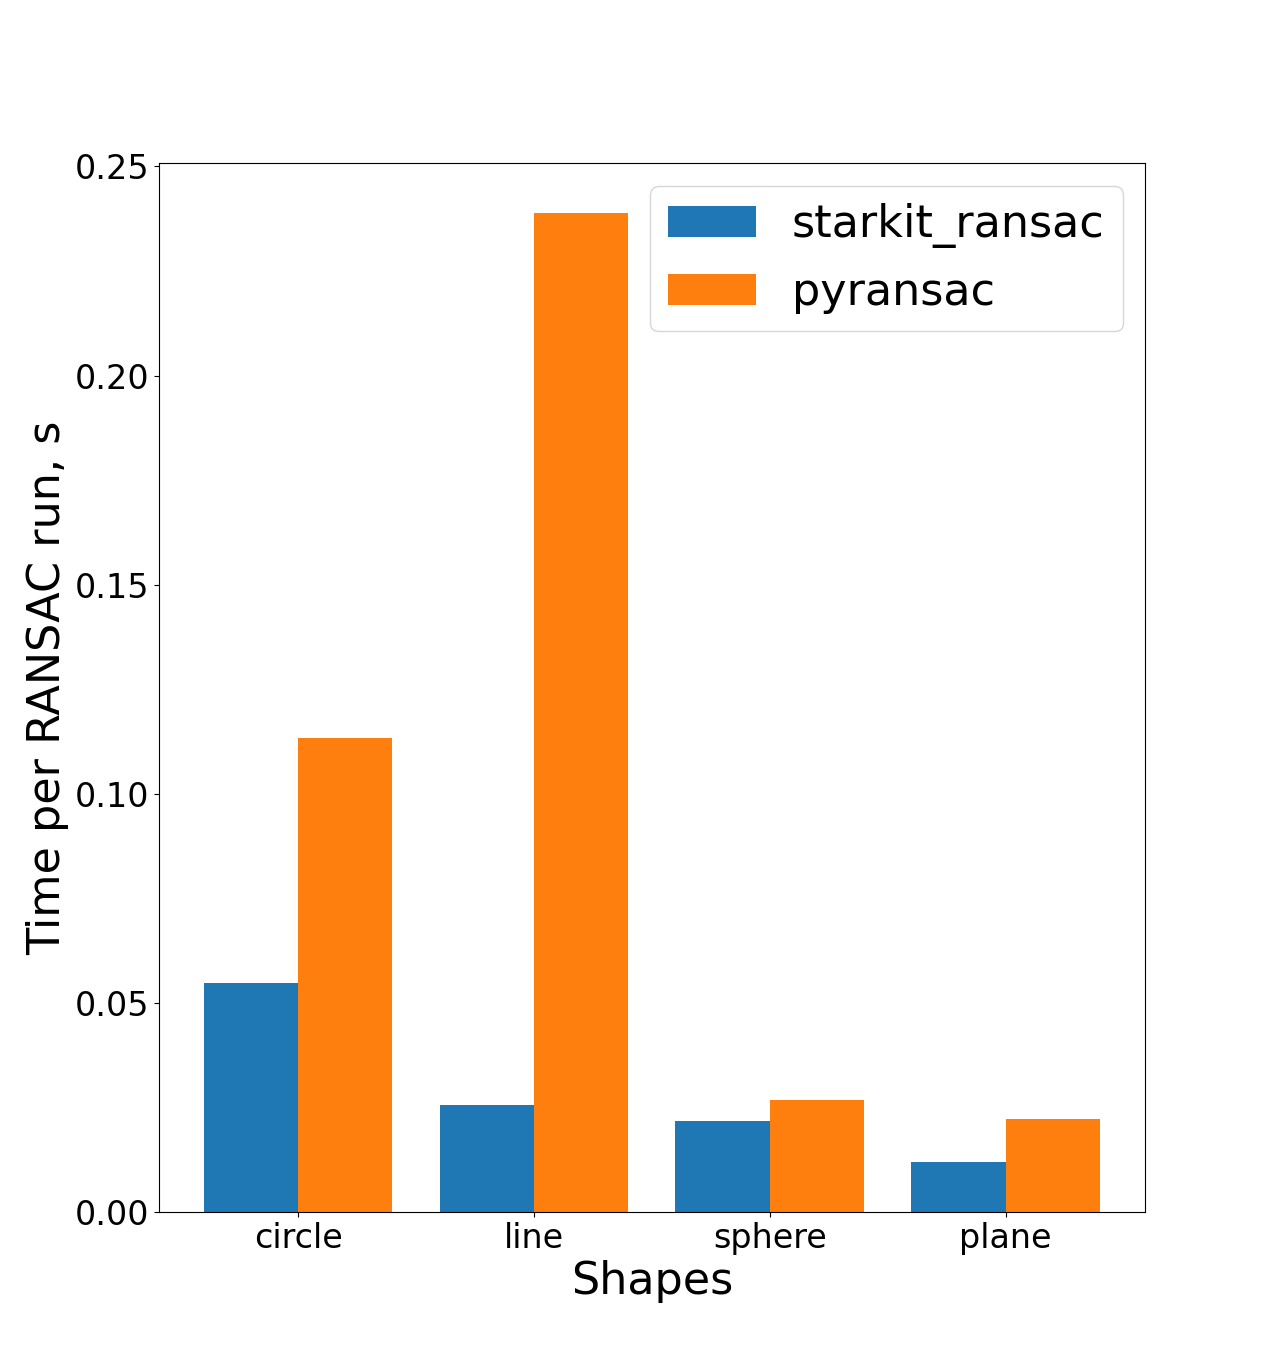
\includegraphics{figures/pyransac-comparison.png}}
\caption{Example of a figure caption. \textit{(figure caption).}}
\label{fig}
\end{figure}


\printbibliography
% \begin{thebibliography}{00}
% \bibitem{b1} G. Eason, B. Noble, and I. N. Sneddon, ``On certain integrals of Lipschitz-Hankel type involving products of Bessel functions,'' Phil. Trans. Roy. Soc. London, vol. A247, pp. 529--551, April 1955. \textit{(references)}
% \bibitem{b2} J. Clerk Maxwell, A Treatise on Electricity and Magnetism, 3rd ed., vol. 2. Oxford: Clarendon, 1892, pp.68--73.
% \bibitem{b3} I. S. Jacobs and C. P. Bean, ``Fine particles, thin films and exchange anisotropy,'' in Magnetism, vol. III, G. T. Rado and H. Suhl, Eds. New York: Academic, 1963, pp. 271--350.
% \bibitem{b4} K. Elissa, ``Title of paper if known,'' unpublished.
% \bibitem{b5} R. Nicole, ``Title of paper with only first word capitalized,'' J. Name Stand. Abbrev., in press.
% \bibitem{b6} Y. Yorozu, M. Hirano, K. Oka, and Y. Tagawa, ``Electron spectroscopy studies on magneto-optical media and plastic substrate interface,'' IEEE Transl. J. Magn. Japan, vol. 2, pp. 740--741, August 1987 [Digests 9th Annual Conf. Magnetics Japan, p. 301, 1982].
% \bibitem{b7} M. Young, The Technical Writer's Handbook. Mill Valley, CA: University Science, 1989.
% \bibitem{b8}	V. Puzyrev, S. Koric, and S. Wilkin, “Evaluation of parallel direct sparse linear solvers in electromagnetic geophysical problems,” Comput. Geosci., vol. 89, pp.79–87, 2016.
% \end{thebibliography}
\vspace{12pt}
\color{red}
IEEE conference templates contain guidance text for composing and formatting conference papers. Please ensure that all template text is removed from your conference paper prior to submission to the conference. Failure to remove the template text from your paper may result in your paper not being published.

\end{document}
